\section{Conclusion}\label{sec:conclusion}
%
% \begin{figure}[H]
% 	\centering
% 	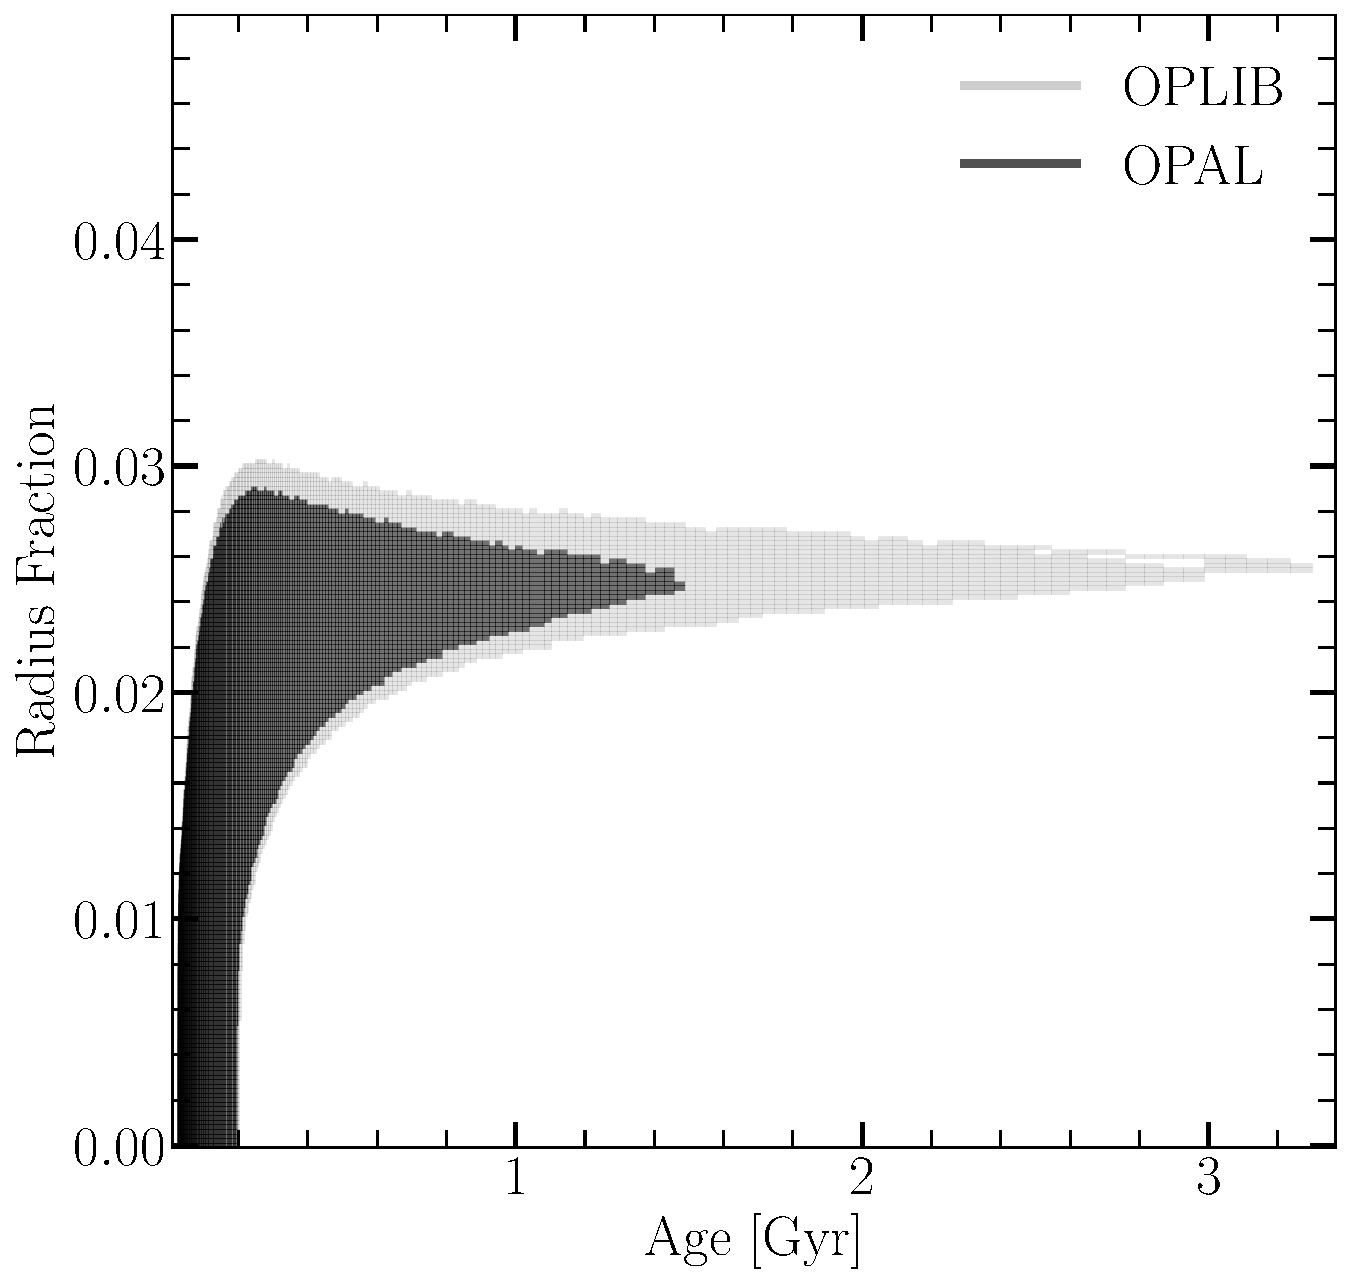
\includegraphics[width=0.45\textwidth]{SameMassConvectiveZoneComp.pdf}
% 	\caption{Portions of 0.3526 $M_{\odot}$ OPAL and OPLIB stellar models
% 	showing the interior shells which are radiative (black region). Note that
% 	for clarity only one convective mixing event from each model is shown. Note
% 	how the radiative zone in the OPLIB model is larger.}
% 	\label{fig:Unstable}
% \end{figure}
%
% \begin{figure}[H]
% 	\centering
% 	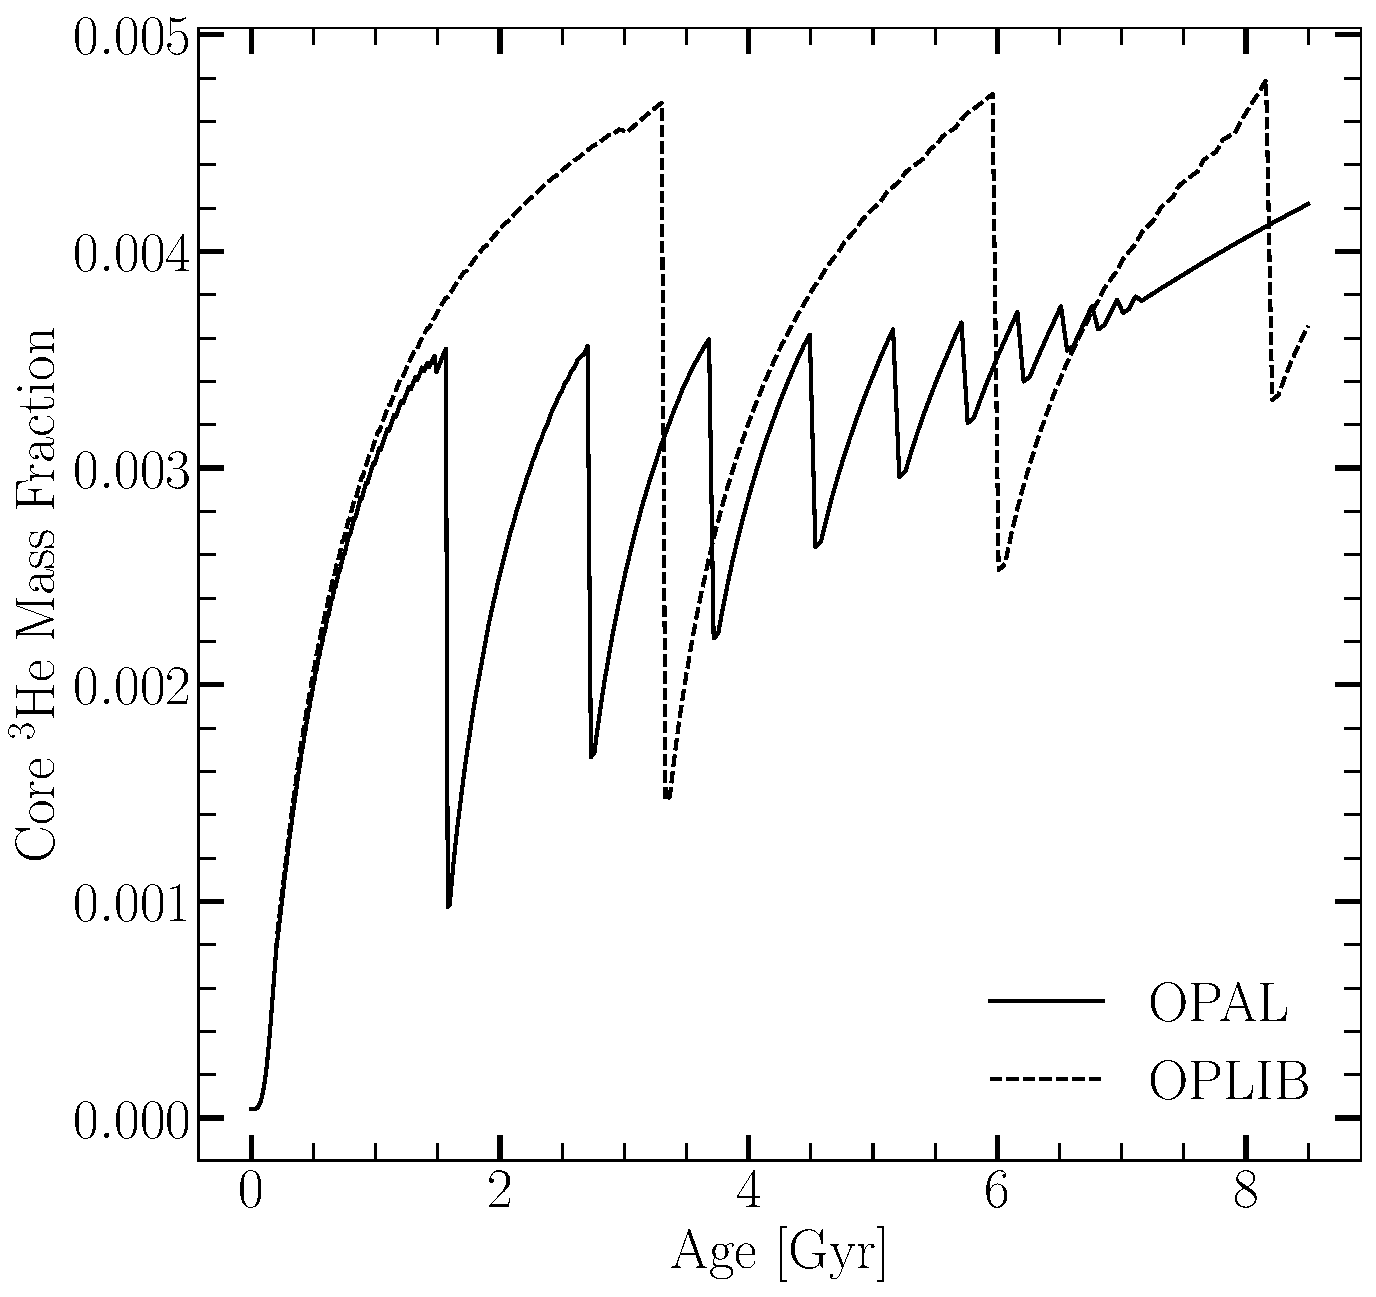
\includegraphics[width=0.45\textwidth]{Core3HECompSameMass.pdf}
% 	\caption{Core $^{3}$He mass fraction for  0.3526 $M_{\odot}$ models evolved
% 	with OPAL and OPLIB (within the Jao Gap's mass range for both). Note how
% 	the OPLIB model's core $^{3}$He mass fraction grows at approximately the
% 	same rate as the OPAL model's but continues uninterrupted for longer.}
% 	\label{fig:OPALOPLIB3He}
% \end{figure}
The Jao Gap provides an intriguing probe into the interior physics of M Dwarfs
stars where traditional methods of studying interiors break down. However,
before detailed physics may be inferred it is essential to have models which
are well matched to observations. Here we investigate whether the OPLIB opacity
tables reproduce the Jao Gap location and structure more accurately than the
widely used OPAL opacity tables. We find that while the OPLIB tables do shift
the Jao Gap location more in line with observations, by approximately 0.05
magnitudes, the shift is small enough that it is likely not distinguishable
from noise due to population age and chemical variation. However, future
measurement of [Fe/H] for stars within the gap will be helpful in constraining
the degree to which the gap should be smeared by these theoretical models.

We also find that both the color and magnitude of the Jao Gap are
correlated to the convective mixing length parameter. Specifically, a lower
mixing length parameter will bring the gap in the populations presented in this
paper more in line with the current best estimate for the actual gap magnitude.
Using this relation it may be possible for mixing length to be calibrated for
low mass stars such that models match the Jao Gap location. Further, the Jao
gap location may provide a test of alternative convection models such as
entropy calibrated convection \citep{Spada2021}. Both of these potential uses
require careful handeling of other uncertanties such as the uncertanties in
bolometric correction, popupulation composition, and population age. As we
currently do not have reason to suspect that the mixing length for the low mass
stars in the DR2 and ERD3 CMD is substantially lower than that of the sun we
leave the investigation of these potential additionl uses for future work.

Finally, we do not find that the OPLIB opacity tables help in reproducing the
as yet unexplained wedge shape of the observed Gap.
